\documentclass{standalone}

\usepackage[utf8]{inputenc}
\usepackage{newtxtext}
\usepackage{newtxmath}
\usepackage[italic]{heppennames}
\usepackage[svgnames]{xcolor}
\usepackage{tikz-feynhand}

\begin{document}
% Very colourful graph to show how colours work.
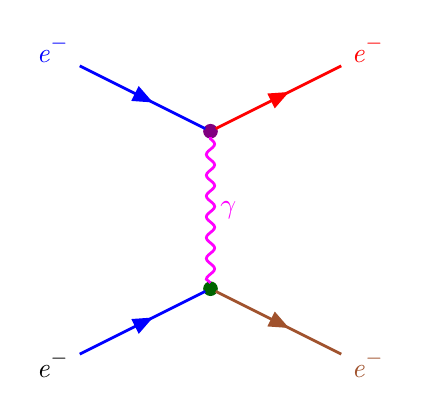
\begin{tikzpicture} 
  \setlength{\feynhandlinesize}{1.0pt}
  \tikzfeynhandset{every fermion={/tikz/color=Sienna}, every dot={/tikz/color=Purple},}
  \begin{feynhand}
    % Define vertices
    \vertex [particle, Blue] (eIn1) at (-2, +2) {\Pem};
    \vertex [particle] (eIn2) at (-2, -2) {\Pem};
    \vertex [particle, Red] (eOut1) at (+2, 2) {\Pem};
    \vertex [particle, Sienna] (eOut2) at (+2, -2) {\Pem};
    \vertex [dot] (eeg1) at (0, +1.0) {};
    \vertex [dot, DarkGreen] (eeg2) at (0, -1.0) {};
    % Lines
    \propagator [fermion, Blue] (eIn1) to (eeg1);
    \propagator [fermion, Red] (eeg1) to (eOut1);
    \propagator [fermion, Blue] (eIn2) to (eeg2);
    \propagator [fermion] (eeg2) to (eOut2);
    \propagator [photon, Magenta] (eeg1) to [edge label = \Pgg] (eeg2) ;
  \end{feynhand}
\end{tikzpicture}
\end{document}
